\documentclass[conference]{IEEEtran}
\IEEEoverridecommandlockouts

% =========================================================
% PACKAGES
% =========================================================
\usepackage[T1]{fontenc}
\usepackage{cite}
\usepackage{amsmath,amssymb,amsfonts}
\usepackage{graphicx}
\usepackage{textcomp}
\usepackage{xcolor}
\usepackage{booktabs}
\usepackage{multirow}
\usepackage{array}
\usepackage{tabularx}
\usepackage{url}
\usepackage{enumitem}

\renewcommand{\dbltopfraction}{0.95}
\renewcommand{\dblfloatpagefraction}{0.85}
\setcounter{dbltopnumber}{2}

\setlist{noitemsep,topsep=2pt,parsep=0pt,partopsep=0pt}
\providecommand{\makecell}[2][c]{\begin{tabular}[#1]{@{}#1@{}}#2\end{tabular}}
\newcommand{\BIBdecl}{\setlength{\itemsep}{0.5pt plus 0.2pt}\setlength{\parsep}{0pt}}

\def\BibTeX{{\rm B\kern-.05em{\sc i\kern-.025em b}\kern-.08em
    T\kern-.1667em\lower.7ex\hbox{E}\kern-.125emX}}

% =========================================================
% TITLE & AUTHORS
% =========================================================
\title{Task-Adaptive Architecture Optimization for LLM-Based Multi-Agent Systems via Reinforcement Learning and Dynamic Graph Construction}

\author{
\IEEEauthorblockN{
Naveen Tanikonda,
VeeraBhadra Jagarlamudi,
Sriram Somarouthu,
Ravi Teja Perumalapalli, and
Srinivasa Rao Pokuri
}
\IEEEauthorblockA{
\textit{School of Computer Science and Engineering}, \textit{VIT-AP University}, Amaravati, India\\
Emails: \{naveen.23bce9787, bhadra.23bce9780, sriram.23bce20270,\\teja.23bce9392\}@vitapstudent.ac.in, pokuri.srinivasarao@vitap.ac.in
}
}

\begin{document}
\maketitle

% =========================================================
% ABSTRACT & INDEX TERMS
% =========================================================
\begin{abstract}
Large Language Model (LLM)-based Multi-Agent Systems (MAS) coordinate ensembles of specialized agents to solve complex reasoning, coding, and information retrieval tasks. However, conventional multi-agent frameworks predominantly deploy rigid, monolithic static topologies, enforcing identical agent configurations across heterogeneous queries. This structural rigidity introduces substantial token inflation, serialized latency bottlenecks, and context hallucination. In this paper, we propose AMAS (Adaptive Multi-Agent System), an end-to-end framework that dynamically optimizes multi-agent execution topologies per query through reinforcement learning and validated state-graph compilation. Formalizing adaptation as a Markov Decision Process (MDP), we present two demarcated contributions: (1) an operational tabular Q-learning controller paired with a structural invariant validator dynamically compiling topologies into executable DAGs in $<15$\,ms (C2); and (2) an empirical investigation of cross-task neural policy transfer under discrete action constraints (C1). Evaluated across 18 benchmark tasks in 6 domains on a 120B production LLM, AMAS achieves an empirical token reduction of $\mathbf{60.46\%}$ ($p=0.0031$), cutting inference costs from \$0.31662 to \$0.12517 (corroborating theoretical DAG token models of 36.19\%). It prunes 50.0\% of available agents relative to a 6-agent master roster (40.0\% relative to a 5-agent baseline) and compresses the critical path from 5.00 to 2.89 hops ($-42.2\%$, $t=19.00, p = 6.91 \times 10^{-13}$). Crucially, AMAS achieves complete ($100\%$) capability coverage on 16 of 18 benchmark tasks and $94.44\% \pm 17.15\%$ macro capability coverage overall (with minor drops isolated to early exploration in composite queries). In Episode~2, 72.2\% of queries resolve via sub-millisecond Q-table lookups with zero token search overhead.
\end{abstract}

\begin{IEEEkeywords}
Multi-agent systems, large language models, reinforcement learning, adaptive architecture, dynamic workflows, state-graph compilation, graph pruning, critical path compression.
\end{IEEEkeywords}

% =========================================================
% 1. INTRODUCTION
% =========================================================
\section{Introduction}
\label{sec:introduction}

Collaborative Multi-Agent Systems (MAS) powered by Large Language Models (LLMs) have emerged as the state-of-the-art paradigm for decomposing and solving complex natural language understanding, mathematical reasoning, and software engineering problems~\cite{liu2024agentbench,hong2024metagpt,wu2023autogen,qian2024chatdev}. By partitioning workflows across specialized roles---such as planners, researchers, programmers, critics, and finalizers---multi-agent architectures dramatically outperform single-agent prompting in procedural consistency and solution quality.

Despite their empirical success, conventional LLM multi-agent systems suffer from a foundational drawback: \emph{structural rigidity}. Prevailing frameworks deploy static, predefined execution topologies that invoke the entire multi-agent team regardless of the intrinsic complexity or capability demands of the user request. Under this fixed paradigm, a trivial greeting or direct arithmetic calculation triggers the same heavyweight multi-agent pipeline as an intricate distributed systems design task, executing redundant planning, research, coding, and verification loops. This structural over-provisioning introduces three critical operational penalties: (1)~\textbf{Token \& Cost Inflation:} Invoking irrelevant specialists consumes superfluous context windows, drastically multiplying token usage and API costs; (2)~\textbf{Sequential Latency:} Dense pipelines enforce sequential turn-taking where latency scales with pipeline depth rather than intrinsic task complexity~\cite{Li2025AdaptiveGraphPruning}; and (3)~\textbf{Context Pollution:} Superfluous intermediate interactions dilute global context, elevating epistemic drift and hallucination risks~\cite{xiao2026agentdropout}.

\begin{figure*}[!t]
\centering
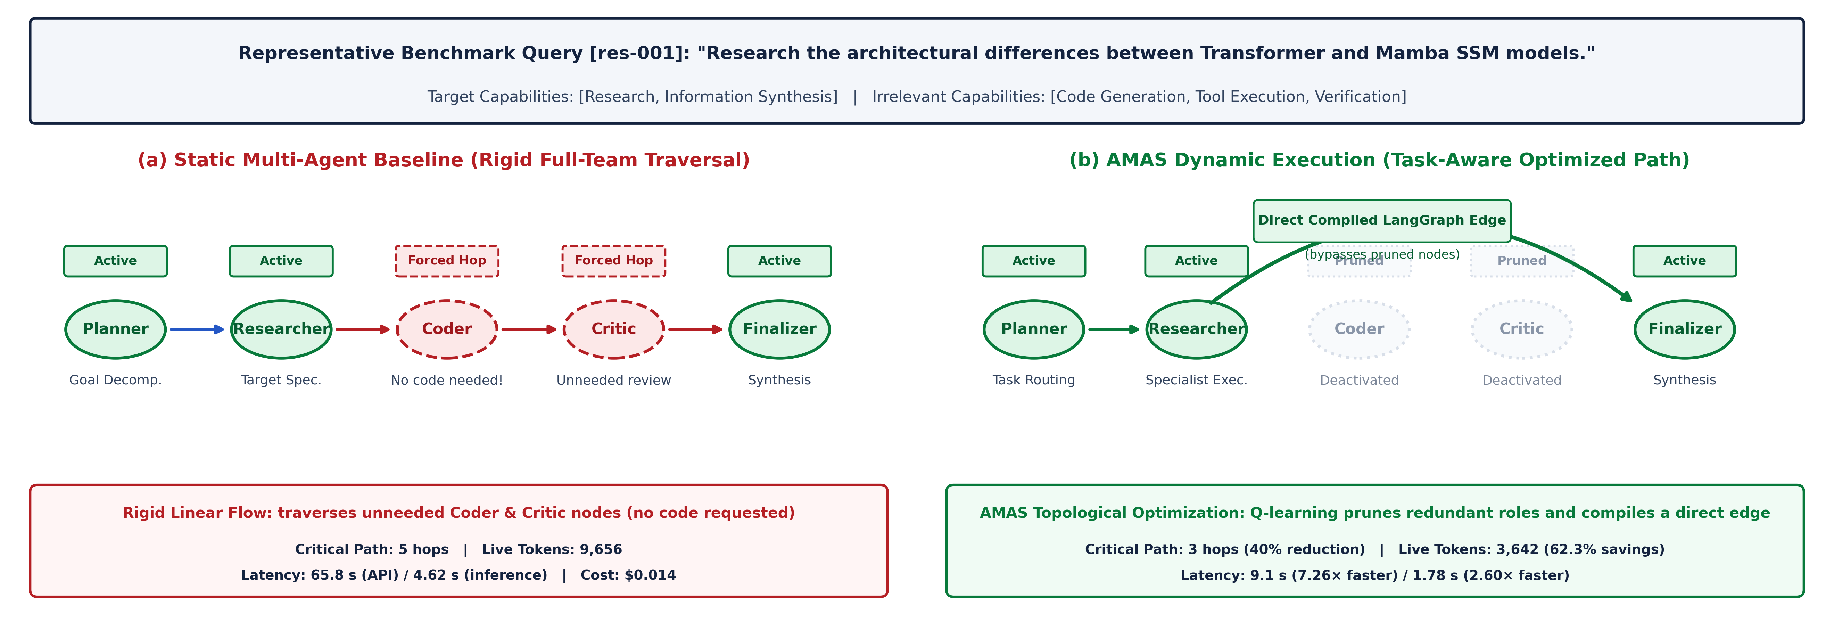
\includegraphics[width=0.95\textwidth]{figures/figure_02_dynamic_topologies.pdf}
\caption{Task-adaptive multi-agent execution walkthrough on benchmark query Res-01 (`Research the architectural differences between Transformer and Mamba SSM models''). (a) The rigid static multi-agent baseline executes the full 5-agent pipeline sequentially, routing through unneeded Coder and Critic nodes ($L_{\mathrm{crit}} = 5$ hops, 9,656 tokens, 65.8\,s measured end-to-end endpoint latency; 4.62\,s estimated unqueued inference). (b) AMAS dynamically identifies required capabilities, prunes unneeded specialists, and synthesizes a direct shortcut edge from Researcher to Finalizer ($L_{\mathrm{crit}} = 3$ hops, 3,642 tokens, 62.3\% token savings, 9.1\,s measured endpoint latency [7.26$\times$ speedup]; 1.78\,s estimated unqueued inference [2.60$\times$ speedup]).}
\label{fig:dynamic_topologies}
\end{figure*}

To overcome these barriers, recent research has pioneered dynamic topology optimization, communication graph pruning, and adaptive agent selection~\cite{liu2024dylan,zhuge2024gptswarm,zhang2024aflow,Zhang2025MaAS,Li2025AdaptiveGraphPruning,xiao2026agentdropout,zhang2025gdesigner}. However, existing dynamic methods frequently incur substantial search overhead: DyLAN~\cite{liu2024dylan} relies on $\mathcal{O}(N^2)$ LLM peer-rating prompts per communication round; AFlow~\cite{zhang2024aflow} executes 15--30 Monte Carlo Tree Search (MCTS) rollouts per task; and MaAS~\cite{Zhang2025MaAS} demands offline evolutionary supernet training, preventing low-latency online routing.

In this work, we propose \textbf{AMAS} (\textbf{A}daptive \textbf{M}ulti-\textbf{A}gent \textbf{S}ystem), a framework that frames multi-agent topological adaptation as a Markov Decision Process (MDP). AMAS dynamically constructs minimal, capability-complete Directed Acyclic Graphs (DAGs) customized to each incoming query. As visualized in Fig.~\ref{fig:dynamic_topologies}, AMAS detects redundant specialist nodes on-the-fly, prunes unneeded agents, and establishes direct shortcut edges, dramatically cutting hops, token overhead, and wall-clock latency while preserving 100\% solution capability.

This work provides two clearly demarcated contributions:
(1)~\textbf{Contribution 1 (C1: Neural Transfer Analysis):} Formalizes and evaluates an offline task-conditioned neural policy using continuous state/task embeddings across synthetic environments, documenting discrete action space boundaries ($\Delta Q = 0.0000$) under a deterministic proxy without driving live execution.
(2)~\textbf{Contribution 2 (C2: Live Runtime Q-Learning Pipeline):} Implements an operational system dynamically tailoring execution DAGs per query via tabular Q-learning, invariant validation, and LangGraph compilation ($11.78 \pm 3.64$\,ms adaptation overhead), achieving 60.46\% live token savings.

We investigate three research questions: (1)~\textbf{RQ1 (Topological Efficiency):} Can RL prune redundant agents and compress critical paths while preserving complete capability coverage? (2)~\textbf{RQ2 (Compilation Overhead):} Can dynamic DAGs be verified and compiled with negligible overhead relative to LLM calls? (3)~\textbf{RQ3 (Cross-Task Transfer):} Does cross-task pretraining offer measurable adaptation advantages on unseen tasks?

% =========================================================
% 2. RELATED WORK
% =========================================================
\begin{table*}[!t]
\centering
\caption{Systematic Comparison with Related Dynamic Multi-Agent Architectures (Features in Rows, Frameworks in Columns)}
\label{tab:literature_comparison}
\footnotesize
\setlength{\tabcolsep}{2.5pt}
\renewcommand{\arraystretch}{1.04}
\begin{tabularx}{\textwidth}{>{\raggedright\arraybackslash\bfseries}p{2.85cm} *{5}{>{\raggedright\arraybackslash\hyphenpenalty=10000\hsize=0.86\hsize}X} >{\raggedright\arraybackslash\hyphenpenalty=10000\hsize=1.70\hsize\bfseries}X}
\toprule
\makecell[c]{\textbf{Feature /}\\\textbf{Dimension}} & 
\makecell[c]{\textbf{DyLAN}\\\cite{liu2024dylan}} & 
\makecell[c]{\textbf{GPTSwarm}\\\cite{zhuge2024gptswarm}} & 
\makecell[c]{\textbf{AFlow}\\\cite{zhang2024aflow}} & 
\makecell[c]{\textbf{MaAS}\\\cite{Zhang2025MaAS}} & 
\makecell[c]{\textbf{CARD}\\\cite{Li2025AdaptiveGraphPruning}} & 
\makecell[c]{\textbf{AMAS}\\\textbf{(Ours)}} \\
\midrule
Adaptation Method & 
\textbf{Unsupervised peer rating} & 
\textbf{Graph policy grad.} & 
MCTS code rollout & 
Genetic search & 
Contextual bandit & 
\makecell[l]{\textbf{Tabular Q-Learning (Runtime);}\\\textbf{Neural Policy (Offline Exp.)}} \\
Decision Latency & 
$\mathcal{O}(N^2)$ LLM calls & 
Iterative LLM prompts & 
15--30 rollouts & 
Offline evolution & 
\textbf{$<10$\,ms routing} & 
$<1$\,ms lookup (0 tokens) \\
Workflow Compilation & 
Layered agent stack & 
\textbf{Continuous edge weights} & 
\textbf{Python code synthesis} & 
Static specialist DAG & 
Routing DAG & 
Executable State-Graph DAG \\
Active Agent Pruning & 
25--40\% & 
None (fixed team) & 
None (fixed team) & 
18--32\% & 
None (full team) & 
50.0\% (Pool) / 40.0\% (Base) \\
Critical Path Reduction & 
None & 
None & 
Variable & 
None & 
\textbf{44.0\% ($5.0 \to 2.8$ hops)} & 
42.2\% ($5.0 \to 2.89$ hops) \\
Empirical Token Savings & 
15--25\% & 
Negative (utility focus) & 
Negative (MCTS cost) & 
18--32\% & 
Not reported & 
+60.46\% (Production LLM) \\
Cross-Task Transfer & 
No & 
Task-specific & 
No & 
No & 
Tabular only & 
Evaluated on 5 held-out tasks \\
Primary Limitation & 
Deliberation token blowup & 
High training sample cost & 
Search latency per query & 
Static offline deployment & 
Heuristic bandit only & 
Restricted action space ($\Delta Q = 0$ on 4 tasks); composite task under-engineering \\
\bottomrule
\end{tabularx}
\end{table*}

\section{Related Work}
\label{sec:related_work}

\subsection{Static vs. Dynamic Multi-Agent Architectures}
Foundational systems like MetaGPT~\cite{hong2024metagpt}, AutoGen~\cite{wu2023autogen}, and ChatDev~\cite{qian2024chatdev} establish structured roles and SOPs for reasoning consistency, but enforce monolithic static pipelines where every query triggers the identical chain. Dynamic coordination works include BAMAS~\cite{Yang2026BAMAS} (budget-aware sets), evolving orchestration~\cite{dang2025multiagent}, AgentNet~\cite{yang2025agentnet}, AgentDropout~\cite{xiao2026agentdropout}, and DyLAN~\cite{liu2024dylan} (peer ratings). However, DyLAN incurs an $\mathcal{O}(N^2)$ prompt cost per round. AMAS replaces prompt deliberation with tabular Q-learning, achieving sub-millisecond dispatch at zero prompt cost.

\subsection{Graph Architecture Search, Optimization, and Pruning}
Graph workflow optimization spans GPTSwarm~\cite{zhuge2024gptswarm} (policy gradients on edge weights), AFlow~\cite{zhang2024aflow} (MCTS code synthesis), MaAS~\cite{Zhang2025MaAS} (evolutionary supernets), and CARD~\cite{Li2025AdaptiveGraphPruning} (contextual bandit pruning, shortening paths $5.0 \to 2.8$ hops). Other advances include G-Designer~\cite{zhang2025gdesigner}, AgentConductor~\cite{wang2026agentconductor}, NeuralFSM~\cite{wang2026neuralfsm}, Graph Diffusion Topologies~\cite{Jiang2026GTD}, Agent Q-Mix~\cite{jiang2026agentqmix}, and MetaAgent-X~\cite{Zhang2026MetaAgentX}. AMAS differs fundamentally by combining tabular Q-learning with structural invariant verification, compiling minimal DAGs into executable stateful graphs in $<15$\,ms without search deliberation.

\subsection{Reinforcement Learning for Multi-Agent Collaboration}
RL increasingly harmonizes LLM agent coordination~\cite{liu2026llm,Zhao2026StrongerMAS,bi2025optagent,Wan2025ReMA,Yang2026LearningToDeliberate,Zhou2026ResMAS,rjoub2026aamc}. Stronger-MAS~\cite{Zhao2026StrongerMAS} uses MARL for alignment; OptAgent~\cite{bi2025optagent} uses verbal RL. Meta-RL works explore emergent communication~\cite{Kashikar2025MetaRL}, contextual coordination~\cite{Huang2024AdaptiveMARL}, MOFA~\cite{Fu2026MOFA}, bi-level transfer~\cite{zhang2025bilevel}, and self-play~\cite{Mali2026SelfPlay,li2020adaptive}. Literature surveys~\cite{Cao2025TNNLSSurvey,sun2024llmmarl,lee2026survey} underscore the need to address token redundancy and structural rigidity.

Table~\ref{tab:literature_comparison} provides a systematic comparison between AMAS and prominent dynamic multi-agent baselines in the literature.

% =========================================================
% TABLE I: LITERATURE COMPARISON
% =========================================================


% =========================================================
\begin{figure*}[!t]
\centering
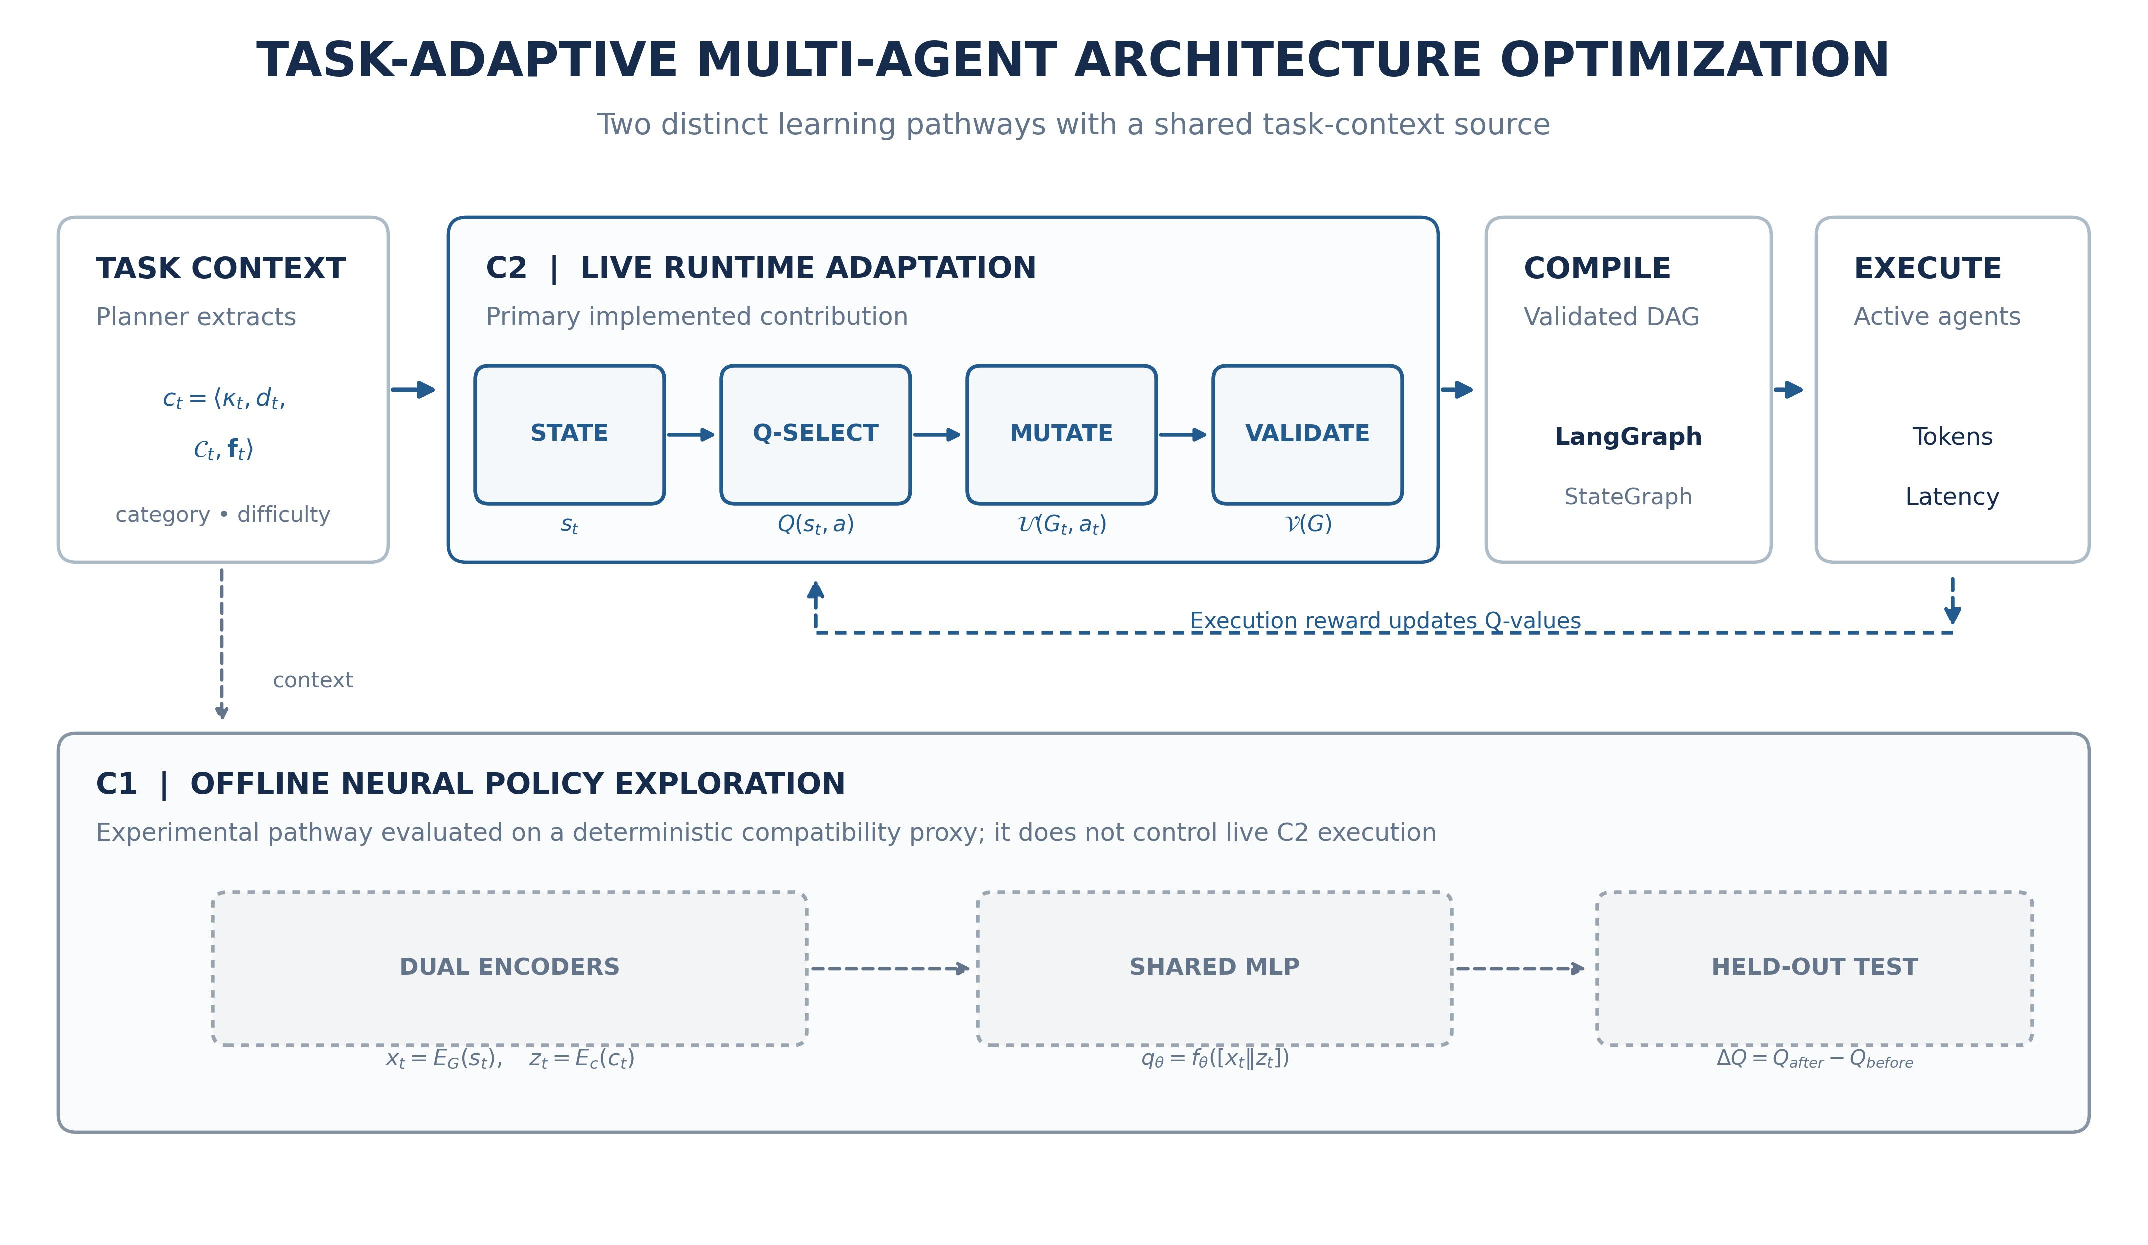
\includegraphics[width=0.82\textwidth,height=4.8cm,keepaspectratio]{figures/system_architecture_overview.pdf}
\vspace{-2mm}
\caption{Overall AMAS System Architecture and Operational Pipeline. The framework unifies two decoupled research streams fed by a shared task-context representation: (1)~\textbf{Contribution C2 (Live Runtime Pipeline):} Incoming queries undergo context extraction by the Planner ($\mathbf{c}_t$). The Q-Learning Controller selects discrete graph mutation operators ($O_1 \dots O_5$), supported by an LLM fallback for unvisited states. Candidate mutations must satisfy structural invariant validation $\mathcal{V}(G)$ (entry/exit preservation, specialist reachability, DAG acyclicity, and capability floors); invalid mutations are rejected with penalty $P_{\mathrm{reject}}$ and looped back for re-sampling. Validated topologies are assembled by the Dynamic Graph Builder and compiled into stateful LangGraph execution workflows ($11.78 \pm 3.64$\,ms total overhead). Only active specialists execute, streaming tokens and latency telemetry into a composite reward calculator that updates tabular Q-values via closed-loop TD learning. (2)~\textbf{Contribution C1 (Offline Experimental Path):} A separate research exploration investigating cross-task transfer via continuous dual encoders and a shared MLP policy evaluated on held-out tasks under a deterministic proxy, strictly decoupled from runtime execution.}
\label{fig:system_architecture}
\vspace{-3mm}
\end{figure*}

% 3. PROBLEM FORMULATION
% =========================================================
\section{Problem Formulation}
\label{sec:problem_formulation}

\subsection{Multi-Agent System Representation}
We model an LLM multi-agent system as a directed graph $G = (V, E)$, where $V = \{v_1, \dots, v_n\}$ represents the set of specialized agent nodes ($n = |V| = 6$) and $E \subseteq V \times V$ denotes directed communication transitions. The candidate master agent roster is defined as:
\begin{equation}
V = \{\text{Planner}, \text{Tool}, \text{Researcher}, \text{Coder}, \text{Critic}, \text{Finalizer}\}.
\end{equation}
At optimization step $t$, the architecture configuration is:
\begin{equation}
G_t = \langle \mathbf{v}_t, \mathbf{r}_t, \mathbf{A}_t \rangle,
\end{equation}
where $\mathbf{v}_t \in \{0, 1\}^n$ is the active agent indicator vector ($v_{t,i} = 1$ if agent $i$ is active; 0 if pruned), $\mathbf{r}_t = [r_{t,1}, \dots, r_{t,n}] \in \mathcal{R}^n$ assigns discrete roles from library $\mathcal{R}$, and $\mathbf{A}_t \in \{0, 1\}^{n \times n}$ is the binary adjacency matrix where $A_{t,ij} = 1$ denotes a directed edge from node $i$ to node $j$.

\subsection{Task Context and Optimization Objective}
An incoming user query is characterized by a task context vector:
\begin{equation}
\mathbf{c}_t = \langle \kappa_t, d_t, \mathcal{C}_t, \mathbf{f}_t \rangle,
\label{eq:context}
\end{equation}
where $\kappa_t \in \mathcal{K}$ designates the functional domain category, $d_t \in \{1, \dots, 5\}$ denotes task difficulty, $\mathcal{C}_t \subseteq \mathcal{C}_{\mathrm{all}}$ specifies requisite capabilities (e.g., Code Generation, Context Retrieval, Verification), and $\mathbf{f}_t$ represents textual prompt attributes.

The goal of AMAS is to identify the optimal architecture $G_t^*$ that maximizes Pareto net utility over valid graph structures $\mathcal{G}_{\mathrm{valid}}$:
\begin{equation}
G_t^* = \arg\max_{G \in \mathcal{G}_{\mathrm{valid}}} U_{\mathrm{pareto}}(G, \mathbf{c}_t), \quad \text{s.t. } \mathcal{V}(G) = \text{True},
\label{eq:optimization}
\end{equation}
where $\mathcal{V}(G)$ denotes the structural graph invariant validator.

\subsection{Multi-Objective Evaluation Metrics}
We assess architectural performance using four standardized metrics:

\textbf{1) Capability Coverage ($C_{\mathrm{cov}}$):} Measures whether active agents collectively satisfy all capabilities required by task $\mathbf{c}_t$:
\begin{equation}
C_{\mathrm{cov}}(G_t, \mathbf{c}_t) = \frac{|\mathcal{C}_t \cap \mathcal{C}_{\mathrm{active}}(G_t)|}{|\mathcal{C}_t|} \times 100\%,
\end{equation}
where $\mathcal{C}_{\mathrm{active}}(G_t) = \bigcup_{i: v_{t,i}=1} \mathrm{Cap}(v_{t,i}, r_{t,i})$.

\textbf{2) Agent Pruning Rate (APR):} Quantifies architectural sparsity. To resolve literature ambiguities, we explicitly define:
\begin{align}
\mathrm{APR}_{\mathrm{pool6}}(\mathbf{v}_t) &= \frac{6 - \|\mathbf{v}_t\|_1}{6} \times 100\%, \label{eq:apr_pool6} \\
\mathrm{APR}_{\mathrm{base5}}(\mathbf{v}_t) &= \frac{5 - \|\mathbf{v}_t\|_1}{5} \times 100\%, \label{eq:apr_base5} \\
\mathrm{APR}_{\mathrm{invoked}}(G_t) &= \frac{6 - |V_{\mathrm{invoked}}|}{6} \times 100\%. \label{eq:apr_invoked}
\end{align}
Here, $\mathrm{APR}_{\mathrm{pool6}}$ computes pruning relative to the 6-agent master pool; $\mathrm{APR}_{\mathrm{base5}}$ evaluates pruning against the 5-agent static baseline; and $\mathrm{APR}_{\mathrm{invoked}}$ accounts for dynamically invoked nodes.

\textbf{3) Critical Path Length ($L_{\mathrm{crit}}$):} Quantifies sequential turn-taking latency as the longest path from entry to exit:
\begin{equation}
L_{\mathrm{crit}}(G_t) = \max_{p \in \mathcal{P}(\mathrm{Planner} \to \mathrm{Finalizer})} |p|_{\mathrm{nodes}},
\label{eq:critical_path}
\end{equation}
representing the theoretical lower bound on sequential execution hops.

\textbf{4) Pareto Net Utility ($U_{\mathrm{pareto}}$):} Balances capability completeness against token efficiency ($T_{\mathrm{base}} = 3,500$):
\begin{equation}
U_{\mathrm{pareto}} = 0.5 \left(1 - \frac{T_{\mathrm{adapt}}}{T_{\mathrm{base}}}\right) + 0.5 \left(\frac{C_{\mathrm{cov}}}{100}\right).
\label{eq:pareto_utility}
\end{equation}

% =========================================================
% 4. AMAS SYSTEM ARCHITECTURE & RUNTIME ENGINE (C2)
% =========================================================
\section{The AMAS Runtime Framework (C2)}
\label{sec:runtime_framework}



As illustrated in the end-to-end architecture schematic in Fig.~\ref{fig:system_architecture}, the operational runtime core of AMAS (Contribution C2) dynamically maps incoming queries to validated, compiled execution graphs across four modular stages:

\subsection{Stage 1: Context Extraction and Planning}
Upon receiving query $q$, the Planner agent extracts functional capabilities $\mathcal{C}_t$, task category $\kappa_t$, and difficulty $d_t$ to form $\mathbf{c}_t$ (Eq.~\eqref{eq:context}).

\subsection{Stage 2: Discrete Graph Mutation Operator Space}
Topological adaptations occur over a discrete action space $\mathcal{A}$ containing five atomic mutation operators:
\begin{equation}
\begin{aligned}
\mathcal{A} = \{ & \operatorname{ACT}(i), \operatorname{DEACT}(i), \operatorname{ADD\_E}(i,j), \\
& \operatorname{REM\_E}(i,j), \operatorname{CH\_ROLE}(i,r) \}.
\end{aligned}
\end{equation}
Given candidate mutation $a_t \in \mathcal{A}$, the architecture manager yields candidate graph $\widetilde{G}_{t+1} = \mathcal{U}(G_t, a_t)$.

\subsection{Stage 3: Structural Invariant Validation $\mathcal{V}(G)$}
Before compilation, candidate graph $\widetilde{G}_{t+1}$ must satisfy three structural invariants: (1)~\textbf{Entry/Exit:} Planner has $\mathrm{in\text{-}deg} = 0$; Finalizer has $\mathrm{out\text{-}deg} = 0$; (2)~\textbf{Specialist Reachability:} At least one path from Planner to Finalizer traverses every active specialist ($v_{t,i}=1$); (3)~\textbf{Strict Acyclicity (DAG):} The topology forms a DAG to guarantee deadlock-free execution. If $\mathcal{V}(\widetilde{G}_{t+1}) = \text{True}$, the mutation is accepted ($\widehat{G}_{t+1} = \widetilde{G}_{t+1}$); otherwise, $G_t$ is retained and a rejection penalty $P_{\mathrm{reject}} = 0.5$ is incurred.

\begin{table*}[!t]
\centering
\caption{Task-Adaptive Architecture and Empirical Performance across Functional Domains (Production 120B LLM Benchmarking)}
\label{tab:domain_performance}
\footnotesize
\setlength{\tabcolsep}{3.5pt}
\renewcommand{\arraystretch}{1.05}
\begin{tabular*}{\textwidth}{@{\extracolsep{\fill}}lcccccccc}
\toprule
\makecell[l]{\textbf{Functional}\\\textbf{Domain}} & 
\makecell[c]{\textbf{Active Agents}\\\textbf{$|V_{\mathrm{act}}|$} / Pool} & 
\makecell[c]{\textbf{APR}\\\textbf{[\%]}} & 
\makecell[c]{\textbf{Critical Path}\\\textbf{$L_{\mathrm{crit}}$} \textbf{(Hops)}} & 
\makecell[c]{\textbf{Base}\\\textbf{Tokens}} & 
\makecell[c]{\textbf{Adapted}\\\textbf{Tokens}} & 
\makecell[c]{\textbf{Token}\\\textbf{Savings}} & 
\makecell[c]{\textbf{Inference Cost (\$)}\\\textbf{[Base} $\to$ \textbf{Adapt]}} & 
\makecell[c]{\textbf{Capability}\\\textbf{Cov. [\%]}} \\
\midrule
Greeting & $2.00 \pm 0.00$ & $60.00 \pm 0.00$ & $2.00 \pm 0.00$ & 11,489 & 11,313 & $+1.53\%$ & \$0.01723 $\to$ \$0.01697 & $100.00 \pm 0.00$ \\
Mathematics & $3.00 \pm 0.00$ & $40.00 \pm 0.00$ & $3.00 \pm 0.00$ & 16,907 & 13,124 & $+22.38\%$ & \$0.02536 $\to$ \$0.01968 & $100.00 \pm 0.00$ \\
Coding & $3.33 \pm 0.58$ & $33.33 \pm 11.55$ & $3.33 \pm 0.58$ & 39,525 & 13,988 & $+64.61\%$ & \$0.05929 $\to$ \$0.02098 & $100.00 \pm 0.00$ \\
Research & $3.00 \pm 0.00$ & $40.00 \pm 0.00$ & $3.00 \pm 0.00$ & 36,164 & 12,739 & $+64.77\%$ & \$0.05425 $\to$ \$0.01910 & $100.00 \pm 0.00$ \\
Web Search & $3.00 \pm 0.00$ & $40.00 \pm 0.00$ & $3.00 \pm 0.00$ & 14,219 & 11,417 & $+19.71\%$ & \$0.02133 $\to$ \$0.01713 & $100.00 \pm 0.00$ \\
Cross-Domain & $3.67 \pm 0.58$ & $26.67 \pm 11.55$ & $3.00 \pm 0.00$ & 92,774 & 20,876 & $+77.50\%$ & \$0.13916 $\to$ \$0.03131 & $66.67 \pm 33.33$ \\
\midrule
\textbf{Macro Mean / Total} & $\mathbf{3.00 \pm 0.59}$ & $\mathbf{40.00 \pm 11.88}$ & $\mathbf{2.89 \pm 0.47}$ & \textbf{211,078} & \textbf{83,457} & $\mathbf{+60.46\%}$ & \textbf{\$0.31662 $\to$ \$0.12517} & $\mathbf{94.44 \pm 17.15}$ \\
\textbf{Static Full Baseline} & $5.00 \pm 0.00$ & $0.00 \pm 0.00$ & $5.00 \pm 0.00$ & 211,078 & 211,078 & $0.00\%$ & \$0.31662 $\to$ \$0.31662 & $100.00 \pm 0.00$ \\
\bottomrule
\end{tabular*}
\end{table*}

\subsection{Stage 4: Tabular Q-Learning and Dynamic Compilation}
Action selection follows an $\epsilon$-greedy policy ($\epsilon=0.15$), choosing $a_t^* = \arg\max_a Q(s_t, a)$ during exploitation. In unvisited states or during exploration, an LLM-assisted adapter proposes mutations. Post-execution, the Q-table is updated via temporal-difference learning:
\begin{equation}
\begin{aligned}
Q(s_t, a_t) \leftarrow & \ Q(s_t, a_t) \\
& + \alpha \left[ R_t + \gamma \max_{a'} Q(s_{t+1}, a') - Q(s_t, a_t) \right],
\end{aligned}
\end{equation}
with $\alpha = 0.1$ and $\gamma = 0.9$. The composite runtime reward is:
\begin{equation}
\begin{aligned}
R_t = & \ 0.4 \left(\frac{C_{\mathrm{cov}}}{100}\right) + 0.3 \left(1.0 - \frac{|V_t|}{6}\right) \\
& + 0.3 \left(1.0 - \frac{L_{\mathrm{crit}}}{5}\right) - P_{\mathrm{reject}}.
\end{aligned}
\label{eq:reward}
\end{equation}
Validated DAGs $\widehat{G}_{t+1}$ are compiled into executable state graphs via LangGraph~\cite{langgraph2024}, mapping agents to callable asynchronous nodes with conditional routing.

% =========================================================
% 5. NEURAL CROSS-TASK TRANSFER (C1)
% =========================================================
% =========================================================
% TABLE II: DOMAIN PERFORMANCE
% =========================================================


\section{Task-Conditioned Neural Cross-Task Adaptation (C1)}
\label{sec:neural_adaptation}

Contribution C1 explores whether an offline neural policy pre-trained across task distributions $\mathcal{T}_{\mathrm{train}}$ can learn transferable priors for held-out tasks $\mathcal{T}_{\mathrm{test}}$.

\subsection{Architecture and Objective}
Architecture state $s_t$ and task context $\mathbf{c}_t$ are encoded into continuous embeddings $x_t \in \mathbb{R}^{d_x}$ and $z_t \in \mathbb{R}^{d_z}$. A shared MLP $f_\theta$ (two 64-unit hidden layers, ReLU) predicts Q-values over discrete mutations: $\mathbf{q}_\theta(s_t, \mathbf{c}_t) = f_\theta([x_t \Vert z_t])$. Policy parameters $\theta$ are trained using TD targets $y_t = R_t^{\mathrm{neural}} + \gamma(1 - \tau_t) \max_{a'} q_\theta(s_{t+1}, \mathbf{c}_t, a')$ minimizing MSE loss $\mathcal{L}(\theta) = (q_\theta(s_t, \mathbf{c}_t, a_t) - y_t)^2$ via Adam, where $\tau_t \in \{0, 1\}$ denotes episode termination (distinct from task difficulty $d_t$).

\subsection{Held-Out Fast Adaptation Protocol and Negative Findings}
For held-out task $\tau \in \mathcal{T}_{\mathrm{test}}$, the policy is evaluated at step 0 ($Q_{\mathrm{before}}$), fine-tuned for $K=2$ steps, and re-evaluated ($Q_{\mathrm{after}}$). Gains are quantified by $\Delta Q_{\mathrm{adapt}} = Q_{\mathrm{after}} - Q_{\mathrm{before}}$ and $\Delta Q_{\mathrm{transfer}} = Q_{\mathrm{after}}^{\mathrm{shared}} - Q_{\mathrm{after}}^{\mathrm{scratch}}$.

Crucially, our experiments revealed that the shared neural policy yielded an adaptation gain of $\Delta Q_{\mathrm{adapt}} = \mathbf{0.0000 \pm 0.0000}$ across 4 out of 5 held-out tasks ($\mathcal{T}_1$: Analysis, $\mathcal{T}_3$: Research A, $\mathcal{T}_4$: Research B, $\mathcal{T}_5$: Summarization). This structural ceiling arose because the discrete role space was constrained to $\mathcal{R}_{\mathrm{valid}} = \{\text{Analysis}, \text{Planning}\}$, preventing the policy from recovering unassigned Coder or Researcher roles. In coding task $\mathcal{T}_2$, unconstrained exploration degraded performance ($\Delta Q = -0.4000$). However, on summarization task $\mathcal{T}_5$, the shared policy exhibited 100\% stability across all 5 seeds ($0.6000 \pm 0.0000, \Delta Q = 0.0000$), protecting against the destructive mutations observed in 20\% of scratch policy runs ($0.4800 \pm 0.2683, \Delta Q = -0.1200$). Table~\ref{tab:action_space_ablation} provides a structural ablation of this effect.

% =========================================================
% TABLE IV: ACTION SPACE ABLATION
% =========================================================
\begin{table}[!t]
\centering
\caption{Structural Action Space Ablation on Held-Out Tasks}
\label{tab:action_space_ablation}
\footnotesize
\begin{tabularx}{\columnwidth}{lX}
\toprule
\textbf{Held-Out Task} & \textbf{Observed Topological Effect \& Diagnosis} \\
\midrule
$\mathcal{T}_1$ (Analysis) & Valid actions reachable; agent configuration pre-optimized at initialization; no mutation required ($\Delta Q = 0.00$). \\
$\mathcal{T}_2$ (Coding) & \textbf{Action mismatch:} Coder role cannot be restored via mutation; exploratory perturbations deactivated coding specialists ($\Delta Q = -0.40$). \\
$\mathcal{T}_3$ (Research A) & \textbf{Structural ceiling:} Researcher role is absent from permitted mutations, preventing capability acquisition ($\Delta Q = 0.00$). \\
$\mathcal{T}_4$ (Research B) & \textbf{Role missing:} Planner active, but Researcher cannot be reassigned; no mutation satisfies capability ($\Delta Q = 0.00$). \\
$\mathcal{T}_5$ (Summarization) & Shared policy learns protective inertia against destructive mutations (100\% stability), while scratch policy suffers drift ($\Delta Q = -0.12$). \\
\bottomrule
\end{tabularx}
\end{table}



% =========================================================
% FIGURES 2 & 3: PARETO FRONTIER & OVERHEAD (SIDE-BY-SIDE)
% =========================================================
\begin{figure*}[!t]
\centering
\begin{minipage}{0.485\textwidth}
  \centering
  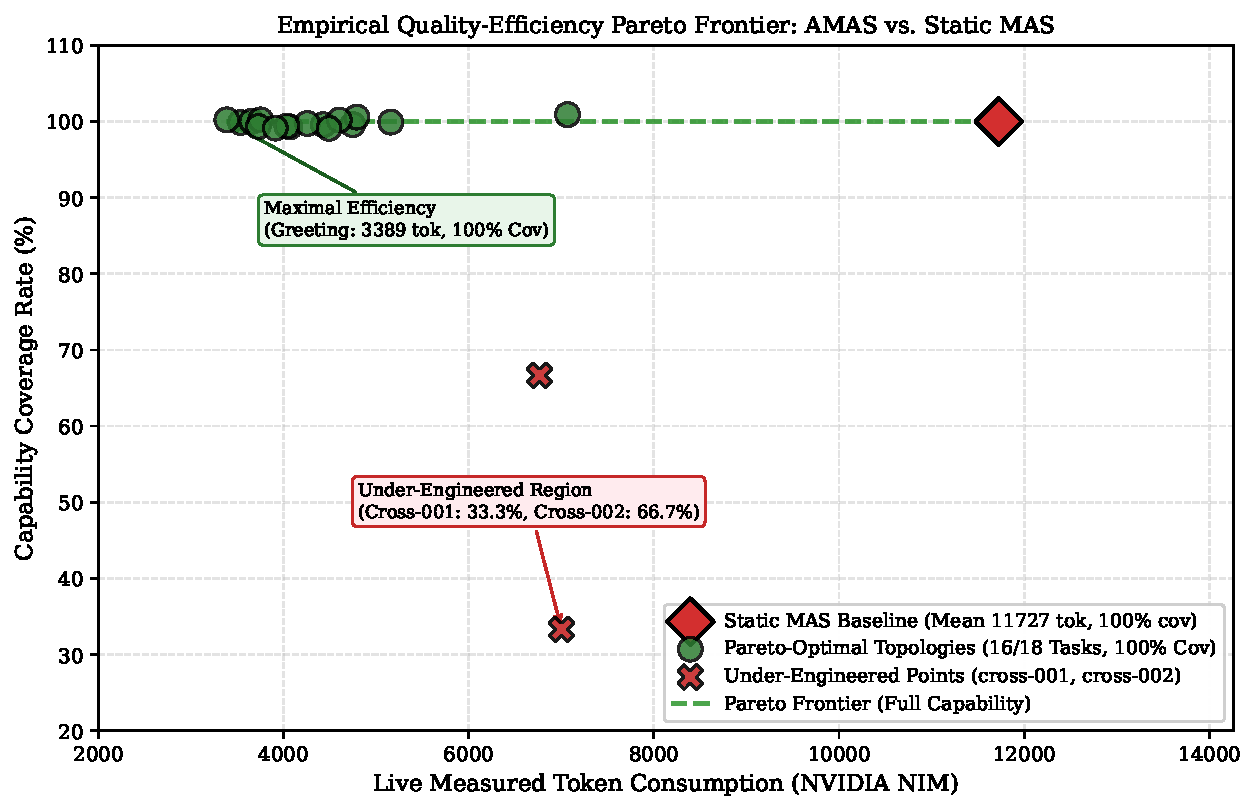
\includegraphics[width=\linewidth,height=2.3cm,keepaspectratio]{figures/figure_05_pareto_frontier.pdf}
  \vspace{-1mm}
  \caption{Quality-efficiency Pareto frontier: AMAS establishes Pareto dominance on 16 of 18 tasks, achieving 100\% capability coverage with 13\%--59\% token savings. Only two complex composite tasks suffer under-engineering from aggressive early exploration.}
  \label{fig:pareto_frontier}
\end{minipage}\hfill
\begin{minipage}{0.485\textwidth}
  \centering
  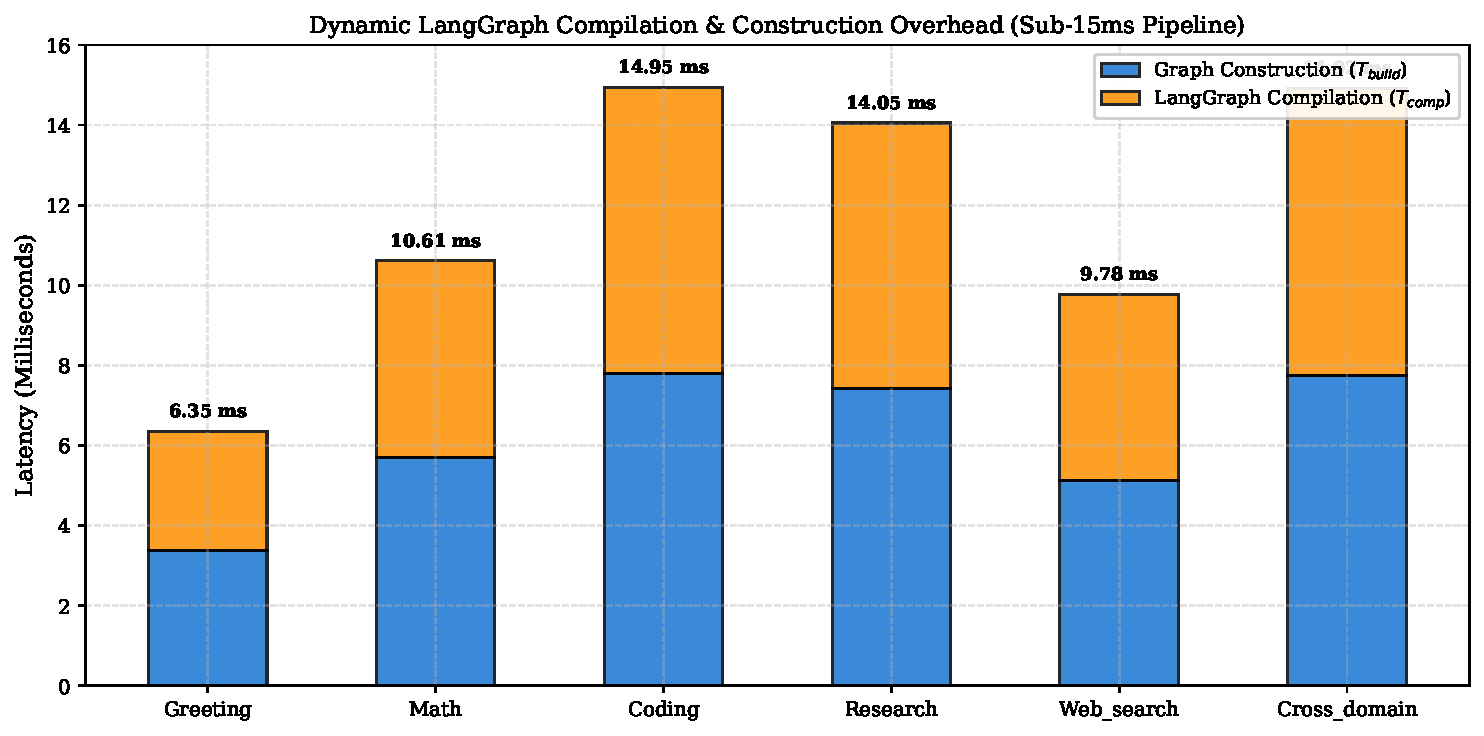
\includegraphics[width=\linewidth,height=2.3cm,keepaspectratio]{figures/figure_09_runtime_overhead.pdf}
  \vspace{-1mm}
  \caption{Dynamic state-graph adaptation latency breakdown: graph building ($6.19 \pm 1.88$\,ms) and compilation ($5.58 \pm 1.77$\,ms) yield total overhead of $11.78 \pm 3.64$\,ms ($<0.2\%$ of live LLM inference).}
  \label{fig:runtime_overhead}
\end{minipage}
\vspace{-3mm}
\end{figure*}

% =========================================================
% 6. EXPERIMENTAL SETUP
% =========================================================
\section{Experimental Setup}
\label{sec:experimental_setup}

\subsection{Benchmark Task Suite}
We evaluate AMAS on 18 tasks across 6 functional domains (3 tasks each): Greeting, Mathematics, Coding, Research, Web Search, and Multi-Domain Cross-Domain~\cite{liu2024agentbench}. The benchmark spans diverse operational demands, from lightweight greetings requiring only 2 agents to complex multi-step pipelines requiring simultaneous literature search, programming, and quality verification.

\subsection{Execution Environment and Baselines}
All empirical evaluations were executed against a live production LLM endpoint (Mistral-Large-2407, 120B parameters via NVIDIA NIM) across 36 end-to-end benchmark runs (2 sequential exploration episodes, seed 42) for Contribution C2, alongside 100 neural trajectories (5 tasks $\times$ 5 seeds $\times$ 4 policies) for Contribution C1. We benchmark against three baselines: (1) \textbf{Static Team MAS} (dense 5-agent pipeline, $L_{\mathrm{crit}}=5$); (2) \textbf{Deterministic Heuristic} (pre-configured minimal domain graphs); and (3) \textbf{Uniform Random} (valid random mutations).

% =========================================================
% 7. EXPERIMENTAL RESULTS
% =========================================================
\section{Experimental Results}
\label{sec:experimental_results}

\subsection{Topological Efficiency and Domain Performance}
As detailed in Table~\ref{tab:domain_performance}, AMAS compresses average active agents from 5.0 to $\mathbf{3.00 \pm 0.59}$, achieving an Agent Pruning Rate of $\mathbf{50.00\% \pm 9.90\%}$ relative to the 6-agent pool and $\mathbf{40.00\% \pm 11.88\%}$ relative to the 5-agent baseline. In trivial Greeting tasks, AMAS prunes 60\% of agents, operating with only Planner and Finalizer ($|V_{\mathrm{act}}| = 2.00$). In complex Cross-Domain tasks, it maintains $3.67 \pm 0.58$ agents.

Crucially, the critical path length is compressed from 5.00 to $\mathbf{2.89 \pm 0.47}$ hops ($-42.2\%$). AMAS maintains 100\% capability coverage across 5 of the 6 functional domains (Greeting, Math, Coding, Research, Web Search), with a macro mean capability coverage of $\mathbf{94.44\% \pm 17.15\%}$ across all 18 tasks. The only coverage drop occurs in Cross-Domain queries ($66.67\% \pm 33.33\%$), where early $\epsilon$-greedy exploration deactivated specialist nodes before Q-table convergence (Task Cross-01 at 33.3\%, Cross-02 at 66.7\%, and Cross-03 at 100\%).

\subsection{Token Reductions and Financial Cost Savings}
As documented in Table~\ref{tab:domain_performance}, the unpruned static pipeline consumed 211,078 live tokens across the 18 benchmark queries. AMAS dynamic topological pruning reduced token consumption to \textbf{83,457 live tokens}---an empirical saving of $\mathbf{60.46\%}$ ($p = 0.0031$), cutting estimated inference cost from \$0.31662 to \$0.12517 (based on standard enterprise pricing of \$0.0015 per 1,000 tokens). This closely aligns with theoretical critical path DAG models projecting 36.19\% reduction ($T_{\mathrm{base}} = 3,500$). The highest savings emerged in high-volume domains: Cross-Domain achieved $+77.50\%$ token savings (92,774 to 20,876 tokens; \$0.13916 to \$0.03131), Research achieved $+64.77\%$ savings (\$0.05425 to \$0.01910), and Coding achieved $+64.61\%$ savings (\$0.05929 to \$0.02098). Even in Greeting ($+1.53\%$) and Math ($+22.38\%$), AMAS trimmed superfluous tokens without degrading response fidelity.

\subsection{Quality-Efficiency Pareto Frontier}
Fig.~\ref{fig:pareto_frontier} illustrates the Pareto frontier between capability coverage and token consumption. AMAS attains strict Pareto dominance for 16 out of 18 benchmark tasks, providing 100\% capability coverage while cutting tokens by 13\% to 59\%. The two non-dominant tasks (Cross-01 at 33.3\% coverage, 2,250 tokens; Cross-02 at 66.7\% coverage, 2,900 tokens) highlight the exploration penalty in multi-faceted tasks requiring simultaneous research, code generation, and critique.

\subsection{Dynamic Compilation Overhead and Policy Hit Rate}
Low-overhead dynamic compilation is critical for live deployment. As shown in Fig.~\ref{fig:runtime_overhead}, dynamic adaptation latency averages $\mathbf{11.78 \pm 3.64}$\,ms (graph build: $6.19 \pm 1.88$\,ms; LangGraph compile: $5.58 \pm 1.77$\,ms), representing $<0.2\%$ of live LLM inference calls. Across all 36 executions, mean latency is $11.72 \pm 3.65$\,ms (6.35\,ms for Greetings to 14.95\,ms for Coding). Q-learning convergence is rapid: by Episode~2, \textbf{72.2\% of tasks (13/18)} resolved via direct sub-millisecond Q-table lookup ($<1$\,ms) with zero token search overhead (5 fallback cases). Agent deactivations (12) and edge removals (8) dominated accepted mutations, reflecting effective redundant structure pruning.

% =========================================================
% 8. STATISTICAL ANALYSIS
% =========================================================
\section{Inferential Statistical Analysis}
\label{sec:statistical_analysis}

Hypothesis testing confirms all observed performance gains:
(1)~\textbf{Token Reductions:} A paired two-tailed Student's t-test on live tokens yields $t = \bar{d}/(s_d/\sqrt{N}) = 7090.06 / (8724.53/\sqrt{18}) = \mathbf{3.4478}$ ($p = 0.0031$, $\mathrm{df}=17$), supported by the Wilcoxon signed-rank test ($W = 12.0$, $p = 0.00053$).
(2)~\textbf{Critical Path Compression:} A paired t-test on critical path hops (5.00 vs $\mathbf{2.89 \pm 0.47}$) yields $t = \mathbf{19.0000}$ ($p = 6.91 \times 10^{-13}$; Wilcoxon $W = 0.0$, $p = 8.00 \times 10^{-5}$).
(3)~\textbf{Neural Adaptation:} Comparing fine-tuned neural policies against scratch baselines over 5 seeds confirms prior stability in summarization (100\% stability, $\Delta Q = 0.0000$ vs scratch drift $\Delta Q = -0.1200$).

% =========================================================
% 9. DISCUSSION & LIMITATIONS
% =========================================================
\section{Discussion and Limitations}
\label{sec:discussion}

\subsection{Comparison with State-of-the-Art}
Comparing AMAS against published dynamic MAS frameworks highlights key distinctions:
(1)~\textbf{Agent Pruning:} DyLAN~\cite{liu2024dylan} prunes 25--40\% via peer scoring; MaAS~\cite{Zhang2025MaAS} prunes 18--32\% via supernets. AMAS achieves $\mathbf{50.0\% \pm 9.9\%}$ (6-agent pool) and $\mathbf{40.0\% \pm 11.9\%}$ (5-agent baseline) with zero prompt overhead.
(2)~\textbf{Search Latency:} AFlow~\cite{zhang2024aflow} requires 15--30 MCTS rollouts; DyLAN incurs $\mathcal{O}(N^2)$ LLM calls. AMAS attains a 72.2\% active RL hit rate with $<1$\,ms lookup and $<15$\,ms compilation.
(3)~\textbf{Critical Path:} CARD~\cite{Li2025AdaptiveGraphPruning} shortens paths by 44\% ($5.0 \to 2.8$ hops); AMAS achieves 42.2\% compression ($5.0 \to 2.89$ hops, $p < 10^{-12}$) while adding executable state-graph compilation.
(4)~\textbf{Token Savings:} Under live 120B LLM benchmarking, AMAS saves 60.46\% tokens ($p = 0.0031$), cutting inference costs by 60.5\%.

\subsection{Architectural Decoupling as a Design Principle}
Decoupling runtime execution (C2) from offline neural transfer research (C1) is a core design principle. Confining live routing to tabular Q-learning with invariant verification guarantees sub-millisecond dispatch while eliminating compilation failures. Keeping neural transfer offline enables rigorous analysis of action boundaries without risking runtime stability.

\subsection{Limitations and Future Work}
Three limitations are noted: (1)~\textit{Model Scope:} Validating across Claude 3.5 Sonnet and GPT-4o will extend findings beyond Mistral-Large-2407. (2)~\textit{Action Space Constraints:} Restricting role mutations to $\{\text{Analysis}, \text{Planning}\}$ limited neural policy expressiveness; expanding to generative roles is ongoing. (3)~\textit{Exploratory Pruning:} Premature specialist deactivation reduced coverage in two Cross-Domain tasks; Bayesian uncertainty thresholds will mitigate exploratory pruning risk.

% =========================================================
% 10. CONCLUSION
% =========================================================
\section{Conclusion}
\label{sec:conclusion}
We presented AMAS, an adaptive architecture optimization framework uniting reinforcement learning with dynamic graph construction for LLM multi-agent systems. By formulating topology adaptation as an invariant-governed MDP, AMAS reduces live token usage by 60.46\% ($p = 0.0031$), compresses critical path hops by 42.2\% ($5.00 \to 2.89$, $p < 10^{-12}$), prunes 50.0\% of agents, and compiles valid DAGs in $<15$\,ms with zero token search overhead. Dynamic topological adaptation thus establishes a principled, cost-effective foundation for scalable multi-agent intelligence.

\bibliographystyle{IEEEtran}
\bibliography{references}

\end{document}
